\documentclass{article}

\usepackage{graphicx} % Für Bilder einfügen
\usepackage{amsmath} % Für mathematische Formeln
\usepackage{hyperref} % Für Hyperlinks
\usepackage{parskip} % Für Absätze
\usepackage{array} % Für Tabellen
\usepackage{amsfonts} % Für mathematische Formeln
\usepackage[utf8]{inputenc} 
\usepackage[ngerman]{babel} 
\usepackage[T1]{fontenc} 
\usepackage{siunitx} %für das Grad Zeichen benötigt
\usepackage{textcomp} 
\usepackage[bottom]{footmisc} % für Fußnote nach unten verschieben
\usepackage{url} % benötigt für URL in Literaturverzeichnis

\title{Abgabe 1 für Computergestützte Methoden}
\author{Gruppe 58, Artur Fast(Matr.-Nr:4081836),\\
Lennart Schröder(Matr.-Nr:4114165), Christoph Hilge(Matr.-Nr:2184017)}
\date{30.11.2024}

\begin{document}

% Title, Autor und Datum erzeugen
\maketitle



% Inhaltsverzeichnis
\tableofcontents

% starte mit dem Inhalt auf der nächsten Seite
\newpage

\section{Der zentrale Grenzwertsatz}
Der zentrale Grenzwertsatz (ZGS) ist ein fundamentales Resultat der Wahrscheinlichkeitstheorie, das die Verteilung von Summen unabhängiger, identisch verteilter (i.i.d.) Zufallsvariablen (ZV) beschreibt. Er besagt, dass unter bestimmten Voraussetzungen die Summe einer großen Anzahl solcher ZV ann"ahernd normalverteilt ist, unabh"angig von der Verteilung der einzelnen ZV. Dies ist besonders n"utzlich, da die Normalverteilung gut untersucht und mathematisch
handhabbar ist.


\subsection{Aussage}
Sei $X_1,X_2,...,X_n$ eine Folge von $i.i.d.$ ZV mit dem Erwartungswert $\mu = \mathbb{E}(X_i)$ und der Varianz $\sigma^2 =$ Var($X_i$), wobei 0 < $\sigma^2$ < $\infty$ gelte. Dann konvergiert die standardisierte Summe $Z_n$ dieser ZV für $n \to \infty$ in Verteilung gegen eine Standardnormalverteilung:\footnote{Der zentrale Grenzwertsatz hat verschiedene Verallgemeinerungen. Eine davon ist der \textbf{Lindeberg-Feller-Zentrale-Grenzwertsatz} [\cite{klenke}, Seite 328], der schw"achere Bedingungen an die Unabh"angigkeit und die identische Verteilung der ZV stellt}
\begin{equation}
    \label{Grenzwertsatz}
    \ Z_n = {\frac{\sum_{i=1}^{n}X_i-n\mu}{\sigma \sqrt{n}}} \xrightarrow{d} \mathcal{N}(0,1).
\end{equation}
Das bedeutet, dass für große $n$ die Summe der ZV näherungsweise normalverteilt ist mit Erwartungswert $n\mu$ und Varianz $n\sigma^2$:
\begin{equation}
\label{zweite Formel}
\sum_{i=1}^{n}X_i\sim \mathcal{N}(n\mu,n\sigma^2).
\end{equation}

\subsection{Erklärung der Standardisierung}
Um die Summe der ZV in eine Standardnormalverteilung zu transformieren, subtrahiert man den Erwartungswert $n\mu$ und teilt durch die Standardabweichung $\sigma\sqrt{n}$. Dies führt zu der obigen Formel \eqref{Grenzwertsatz}. Die Darstellung \eqref{zweite Formel} ist für\\ $n\xrightarrow{}\infty$ nicht wohldefiniert.

\subsection{Anwendungen}
Der ZGS wird in vielen Bereichen der Statistik und der Wahrscheinlichkeitstheorie angewendet. Typische Beispiele sind:
\begin{itemize}
\item Berechnung von Konfidenzintervallen für Stichprobenmittelwerte\cite{studysmarter}
\item Durchführung von Hypothesentests\cite{studysmarter}
\end{itemize}

\newpage
\section{Bearbeitung zur Aufgabe 1}

\subsection{Datenverarbeitung}
\subsubsection{Aufbau des Datensatzes}
In unserem Datensatz geht es um Daten zu einer der vielen Stationen eines Fahrradverleihs. Die uns zugeteilte Station ist die $"$E Fordham Rd ß Webster Ave$"$. Diese Daten beziehen sich auf die Wetterlage und die Anzahl der ausgeliehenen Fahrr"ader im Zeitraum vom 1.1.2023 bis zum 31.12.2023.


Die Attributnamen von A1 bis L1 sind folgende: group, station, date, day\_of\_year, day\_of\_week, month\_of\_year, precipitation, windspeed, min\_temperature, average\_temperature, max\_temperature, count. Ohne die Attributnamen der Zeile 1 haben wir 365 individuelle Zeilen.


Bei der ersten oberflächlichen Betrachtung fällt auf, dass in jeder Spalte (außer in den Spalten A, B und C) einer bis mehrere Attributwerte nicht gegeben sind. Auffallend ist zudem, dass es bei dem Attributnamen max\_temperature einen Attributwert mit -1 gibt, obwohl bei dem Attributnamen min\_temperature der Attributwert \ang{50} Fahrenheit ist. Festzustellen ist auch, dass an wärmeren Tagen meistens mehr Fahrräder ausgeliehen werden als an kalten Tagen, und dass meistens weniger Fahrräder ausgeliehen werden, wenn es regnet. Außerdem spielt auch der Wochentag eine Rolle denn an Montagen werden meistens weniger Fahrräder ausgeliehen als an anderen Tagen der Woche. Festzuhalten ist also, dass die Zahl der ausgeliehenen Fahrräder von der Wetterlage sowie dem Wochentag abhängt.  

\subsubsection{Tabellenkalkulation}

Um unseren Datensatz in Form einer Tabelle besser zu visualisieren importieren wir den Datensatz in eine Tabellenkalkulation (siehe Abbildung \ref{fig:Abb1}).
\begin{figure}[ht]
\centering
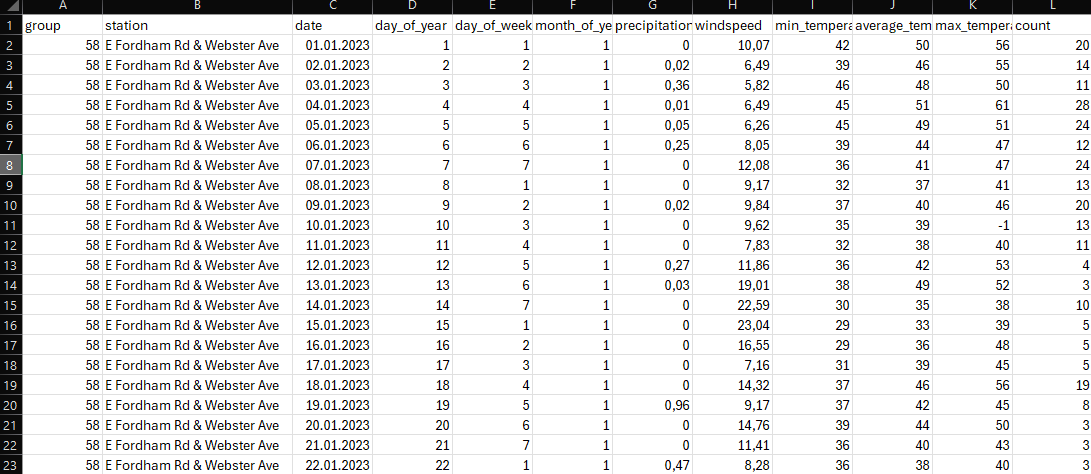
\includegraphics[width = \textwidth]{Abbildung_1.png}
\caption{Tabellenkalkulation}
\label{fig:Abb1}
\end{figure}
\newpage
\subsubsection{Berechnung der höchsten mittleren Temperatur}

Zur Berechnung der höchsten mittleren Temperatur wandeln wir die Tabellenkalkulation in eine Pivot Tabelle (siehe Abbildung \ref{fig:Abb2}) um. Dazu setzen wir in den Wertfeldeinstellungen der durchschnittlichen Temperatur die Wertefelder nach dem maximalen Wert ein. Daraus ergibt sich das Gesamtergebnis von 83 Fahrenheit.


Da wir das Ergebnis jedoch in Celsius brauchen geben wir den folgenden Befehl: =UMWANDELN(G16;"F";"C") in das Feld G17 ein. Nun erhalten wir \ang{28,33333333} Celsius als die höchste mittlere Temperatur.
\begin{figure}[ht]
\centering
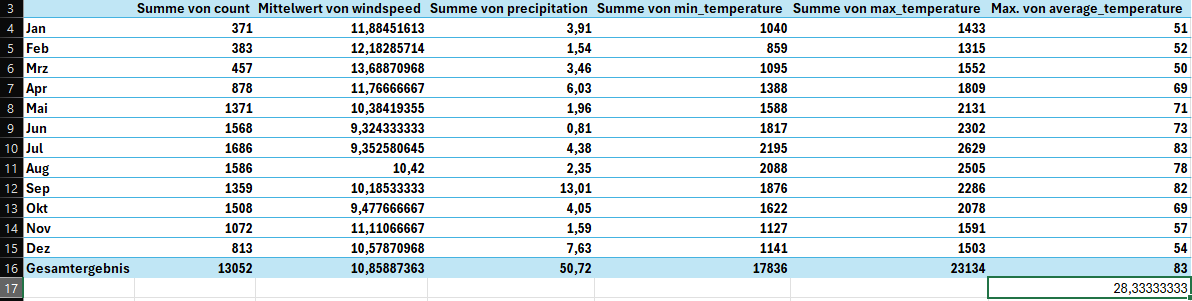
\includegraphics[width = \textwidth]{Abbildung_2.png}
\caption{Pivot Tabelle}
\label{fig:Abb2}
\end{figure}

\subsection{Datenhaltung}

\subsubsection{Normalformen}
Das ist unser Datenbankschema in der 1.ten Normalform:
\begin{tiny}
\begin{center}
\begin{tabular}{|m{3em}|m{1cm}|m{1cm}|m{1cm}|m{1cm}|m{1cm}|m{0,8cm}|m{0,8cm}|m{1cm}|m{1,2cm}|m{1cm}|m{0,5cm}|}
\hline
    group & station & date & day\_of\_ year & day\_of\_ week & month\_of\_ year & precip itation & wind  speed & min\_temp erature & average\_te mperatu re & max\_temp erature & count \\
    \hline
    58 & E Fordham Rd \& Webster Ave & 01.01.2023& 1 & 1 & 1 & 0 & 10,07 & 42 & 50 & 56 & 20 \\
    \hline
\end{tabular}
\end{center}
\end{tiny}
Das ist unser Datenschema in der 2.ten Normalform:
\begin{center}
    \begin{tabular}{|m{2cm}|m{2cm}|m{2cm}|m{2cm}|m{2cm}|m{2cm}|}
    \hline
    \multicolumn{6}{|l|}{Haupttabelle}\\
    \hline
         \underline{ID\#}& gruppe & datum\# & station\_id\# & wetter\_id\# & anzahl \\
         \hline 
    \end{tabular}
\end{center}

\begin{flushleft}
    \begin{tabular}{|m{2cm}|m{2cm}|m{2cm}|m{2cm}|}
    \hline
    \multicolumn{4}{|l|}{Datum}\\
    \hline
        \underline{datum\#} & tag\_jahr & tag\_woche & monat\_jahr  \\
         \hline
    \end{tabular}
\end{flushleft}

\begin{flushleft}
    \begin{tabular}{|m{2cm}|m{2cm}|}
    \hline
    \multicolumn{2}{|l|}{Stationen}\\
    \hline
        \underline{station\_id\#} & station\_name \\
        \hline
    \end{tabular}{}
\end{flushleft}

\begin{center}
    \begin{tabular}{|m{1,8cm}|m{1,8cm}|m{1,8cm}|m{1,8cm}|m{1,8cm}|m{1,8cm}|m{1,8cm}|}
    \hline
    \multicolumn{7}{|l|}{Wetter}\\
    \hline
         \underline{wetter\_id\#}& datum\# & niederschlag & wind & min\_temp & avg\_temp & max\_temp  \\
         \hline
    \end{tabular}{}
\end{center}
Die Werte mit einer Raute sind Attributschlüssel und die Werte mit einer Raute und  Unterstreichung sind Primärschlüssel.

\newpage

\subsubsection{Definition der Tabellen in SQL}

Mit folgendem Code (siehe Abbildung \ref{fig:Abb3}) haben wir die Tabellen mit dem DDL-Teil von SQL definiert.

\begin{figure}[ht]
    \centering
    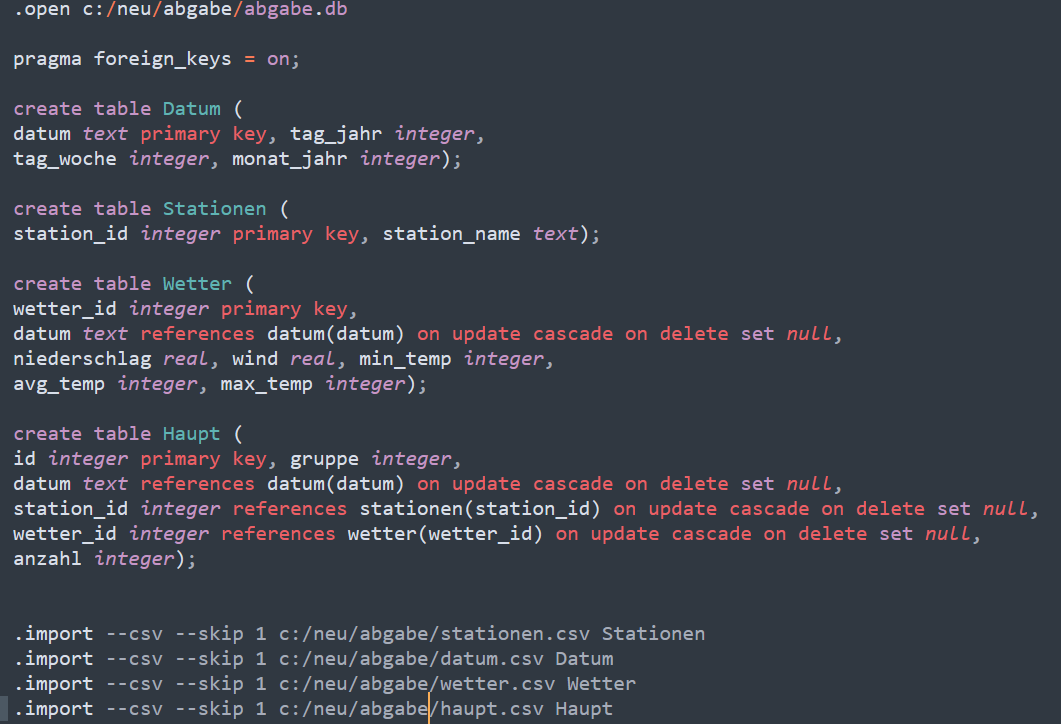
\includegraphics[width= \textwidth]{Abbildung_3.png}
    \caption{Definition der Tabellen}
    \label{fig:Abb3}
\end{figure}

\subsubsection{Vorbereitung des Datensatzes}

Insgesamt haben wir 3 Tabellen in SQL \cite{sqlite} erstellt:

1.Tabelle \glqq bike\grqq{}: Durch Einlesen der Aufgaben-csv (12 Spalten) mit \glqq .import Zielverzeichnis\grqq{}.

2.Tabelle \glqq bike\_id\grqq{}: 12 Spalten aus der 1.Tabelle plus zwei Spalten \glqq id\grqq{} und \glqq station\_id\grqq{} mit der Spalte \glqq id\grqq{} als primary key (so erhält jeder Datensatz eine eindeutige Nummer) mit \glqq create table\grqq{} erstellt.

3.Tabelle \glqq stationen\grqq{} mit den Spalten \glqq station\_id\grqq{} (primary key) und \glqq station\_name\grqq{} erstellt.

Mit 3 SQL-Anweisungen haben wir die Daten aus Tabelle \glqq bike\grqq{} in die entsprechenden Spalten in Tabelle \glqq bike\_id\grqq{} eingelesen und jeder Station eine eindeutige Nummer in der Tabelle \glqq Stationen\grqq{} zugeordnet. Mit dieser Stationsnummer haben wir ein Update der Tabelle \glqq bike\_id\grqq{} gemacht. Das zeigt die\\ Abbildung \ref{fig:Abb4}.

\newpage
\begin{figure}[ht]
    \centering
    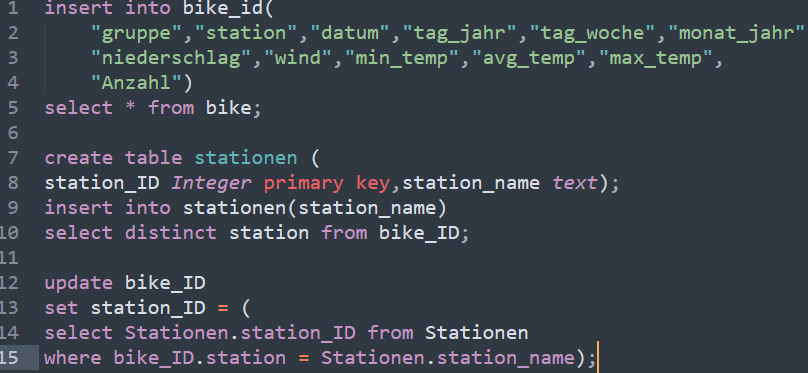
\includegraphics[width= \textwidth]{Abbildung_4.png}
    \caption{Erstellung der Tabellen}
    \label{fig:Abb4}
\end{figure}

Dann haben wir durch 4 Select Anweisungen und den Befehlen \glqq .mode csv\grqq{}, \glqq .mode column\grqq{} und \glqq .once Zielverzeichnis\grqq{} 4 csv-Dateien erstellt, die  unserem Tabellenschema für die 2.Normalform entsprechen.

\begin{figure}[!]
    \centering
    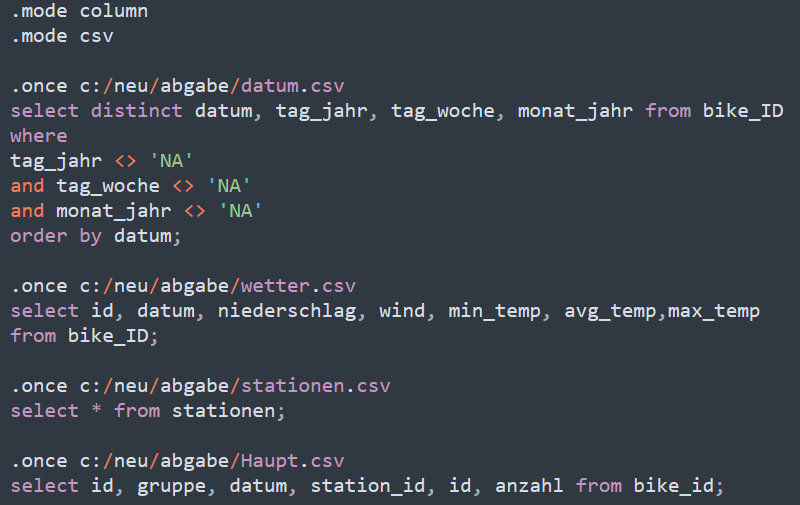
\includegraphics[width= \textwidth]{Abbildung_5.png}
    \caption{Abfragung der csv-Erstellung}
    \label{fig:Abb5}
\end{figure}
\newpage
Durch die Abfrage für das Datum haben wir eine csv-Datei \glqq datum.csv\grqq{} ohne \glqq NA´s\grqq{} erhalten in der jedes Datum aus der ursprünglichen csv-Datei enthalten ist(siehe Abbildung \ref{fig:Abb5}.

In der Abfrage für haupt.csv kommt 2 mal \glqq id\grqq{} vor. Das zweite mal ist für die Spalte \glqq wetter\_id\grqq{}. \glqq id\grqq{} und \glqq wetter\_id\grqq{} sind identisch. Die Spalte soll bei Betrachtung der Haupttabelle darauf hinweisen, dass es Informationen zum Wetter gibt. 

\subsubsection{Abfrage der höchsten mittleren Temperatur}

Die Abfrage zur maximalen mittleren Temperatur haben wir in sqlite3 folgend gelöst(siehe Abbildung \ref{fig:Abb6}) Das Ergebnis der höchsten mittleren Temperatur für unseren Datensatz beträgt \ang{28,3333333333333} Celsius.
\begin{figure}[ht]
    \centering
    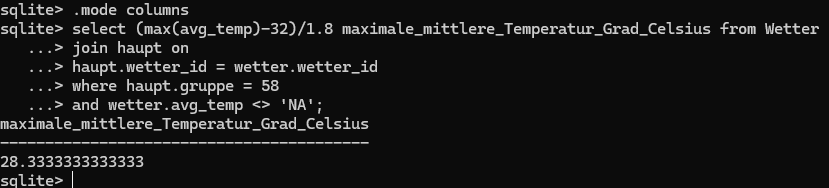
\includegraphics[width= \textwidth]{Abbildung_6.png}
    \caption{Abfrage zur Ermittlung der höchsten mittleren Temperatur}
    \label{fig:Abb6}
\end{figure}

\section{\LaTeX Code}
Der folgende Link stellt den \LaTeX Code bei GitHub zur Verfügung: \url{https://github.com/ArturFast-Ger/Abgabe_1_Comet_Gruppe58.git}


\bibliographystyle{plain}
\bibliography{references}

\end{document}